\documentclass[a4paper]{article}
\usepackage[english]{babel}
\usepackage[utf8]{inputenc}

%
% Graphics
%
\usepackage{graphicx}
\usepackage{xcolor}

\definecolor{alpha}{HTML}{3FA9F5}

%
% Bibliography
%
\usepackage[backend=bibtex,maxnames=5,sorting=none,url=false]{biblatex}
\usepackage{csquotes}

%
% Listings
%
\usepackage{listings}

\definecolor{background}{HTML}{FAFAFA}
\definecolor{sign}{HTML}{3FA9F5}

\lstdefinelanguage{fortune}{
  basicstyle=\ttfamily,
  basewidth={0.5em,0.5em},
  backgroundcolor=\color{background},
  literate=
   *{\%}{{{\color{alpha}{\%}}}}{1}
}

\lstdefinelanguage{shell}{
  basicstyle=\ttfamily,
  basewidth={0.5em,0.5em},
  backgroundcolor=\color{background},
  literate=
    [*]{\\\$}{{{\color{alpha}{\$}}}}{1}
       {Command>}{{{\color{alpha}{Command>}}}}{8}
       {ivan(0)>}{{{\color{alpha}{ivan(0)>}}}}{8}
       {ivan(1)>}{{{\color{alpha}{ivan(1)>}}}}{8}
       {ivan(0):RELEASED>}{{{\color{alpha}{ivan(0):RELEASED>}}}}{17}
       {ivan(0):LOCKED>}{{{\color{alpha}{ivan(0):LOCKED>}}}}{15}
       {ivan(1):LOCKED>}{{{\color{alpha}{ivan(1):LOCKED>}}}}{15}
       {ivan(2):LOCKED>}{{{\color{alpha}{ivan(2):LOCKED>}}}}{15}
}

\lstdefinelanguage{json}{
  basicstyle=\ttfamily,
  basewidth={0.5em,0.5em},
  backgroundcolor=\color{background},
  literate=
   *{:}{{{\color{alpha}{:}}}}{1}
    {,}{{{\color{alpha}{,}}}}{1}
    {\{}{{{\color{alpha}{\{}}}}{1}
    {\}}{{{\color{alpha}{\}}}}}{1}
    {[}{{{\color{alpha}{[}}}}{1}
    {]}{{{\color{alpha}{]}}}}{1}
}

\lstnewenvironment{fortune}%
{\lstset{language=fortune}}%
{}

\lstnewenvironment{json}%
{\lstset{language=json}}%
{}

\lstnewenvironment{shell}%
{\lstset{language=shell}}%
{}

%
% Links
%
\usepackage{hyperref}
\hypersetup{%
  colorlinks=true,
  citecolor={alpha},
  linkcolor={alpha},
  urlcolor ={alpha}
}

%
% Text
%
\newcommand{\ie}{i.e.}
\newcommand{\eg}{e.g.}
\newcommand{\etc}{etc.}

\newcommand{\fix}{should be modified}
\newcommand{\leave}{no changes are needed}
\newcommand{\overwrite}{should contain your previous changes}

\newcommand{\python}{\texttt{Python}}
\newcommand{\classname}[1]{\texttt{#1}}
\newcommand{\filename}[1]{\texttt{#1}}
\newcommand{\code}[1]{\texttt{#1}}

%
% References
%
\newcommand{\sref}[1]{Section~\ref{sec:#1}}
\newcommand{\tref}[1]{Table~\ref{tab:#1}}
\newcommand{\fref}[1]{Figure~\ref{fig:#1}}

\newcommand{\slabel}[1]{\label{sec:#1}}
\newcommand{\tlabel}[1]{\label{tab:#1}}
\newcommand{\flabel}[1]{\label{fig:#1}}

\newcommand{\slab}[1]{\label{sec:#1}}
\newcommand{\tlab}[1]{\label{tab:#1}}
\newcommand{\flab}[1]{\label{fig:#1}}

\newcommand{\aref}[1]{Lab~#1 \cite{description#1}}


\bibliography{include/references.bib}

\title{Distributed Systems: Assignment 4\\Middleware: Distributed Locks}
\author{Petru Eles, Adrian Horga, and Ivan Ukhov\\
\vspace{0.5em}
\href{mailto:petru.eles@liu.se}{petru.eles@liu.se},
\href{mailto:petru.eles@liu.se}{adrian.horga@liu.se}, and
\href{mailto:ivan.ukhov@liu.se}{ivan.ukhov@liu.se}
}
\date{December 20, 2015}

\begin{document}
\maketitle

\section{Introduction}
\begin{figure}
  \centering
  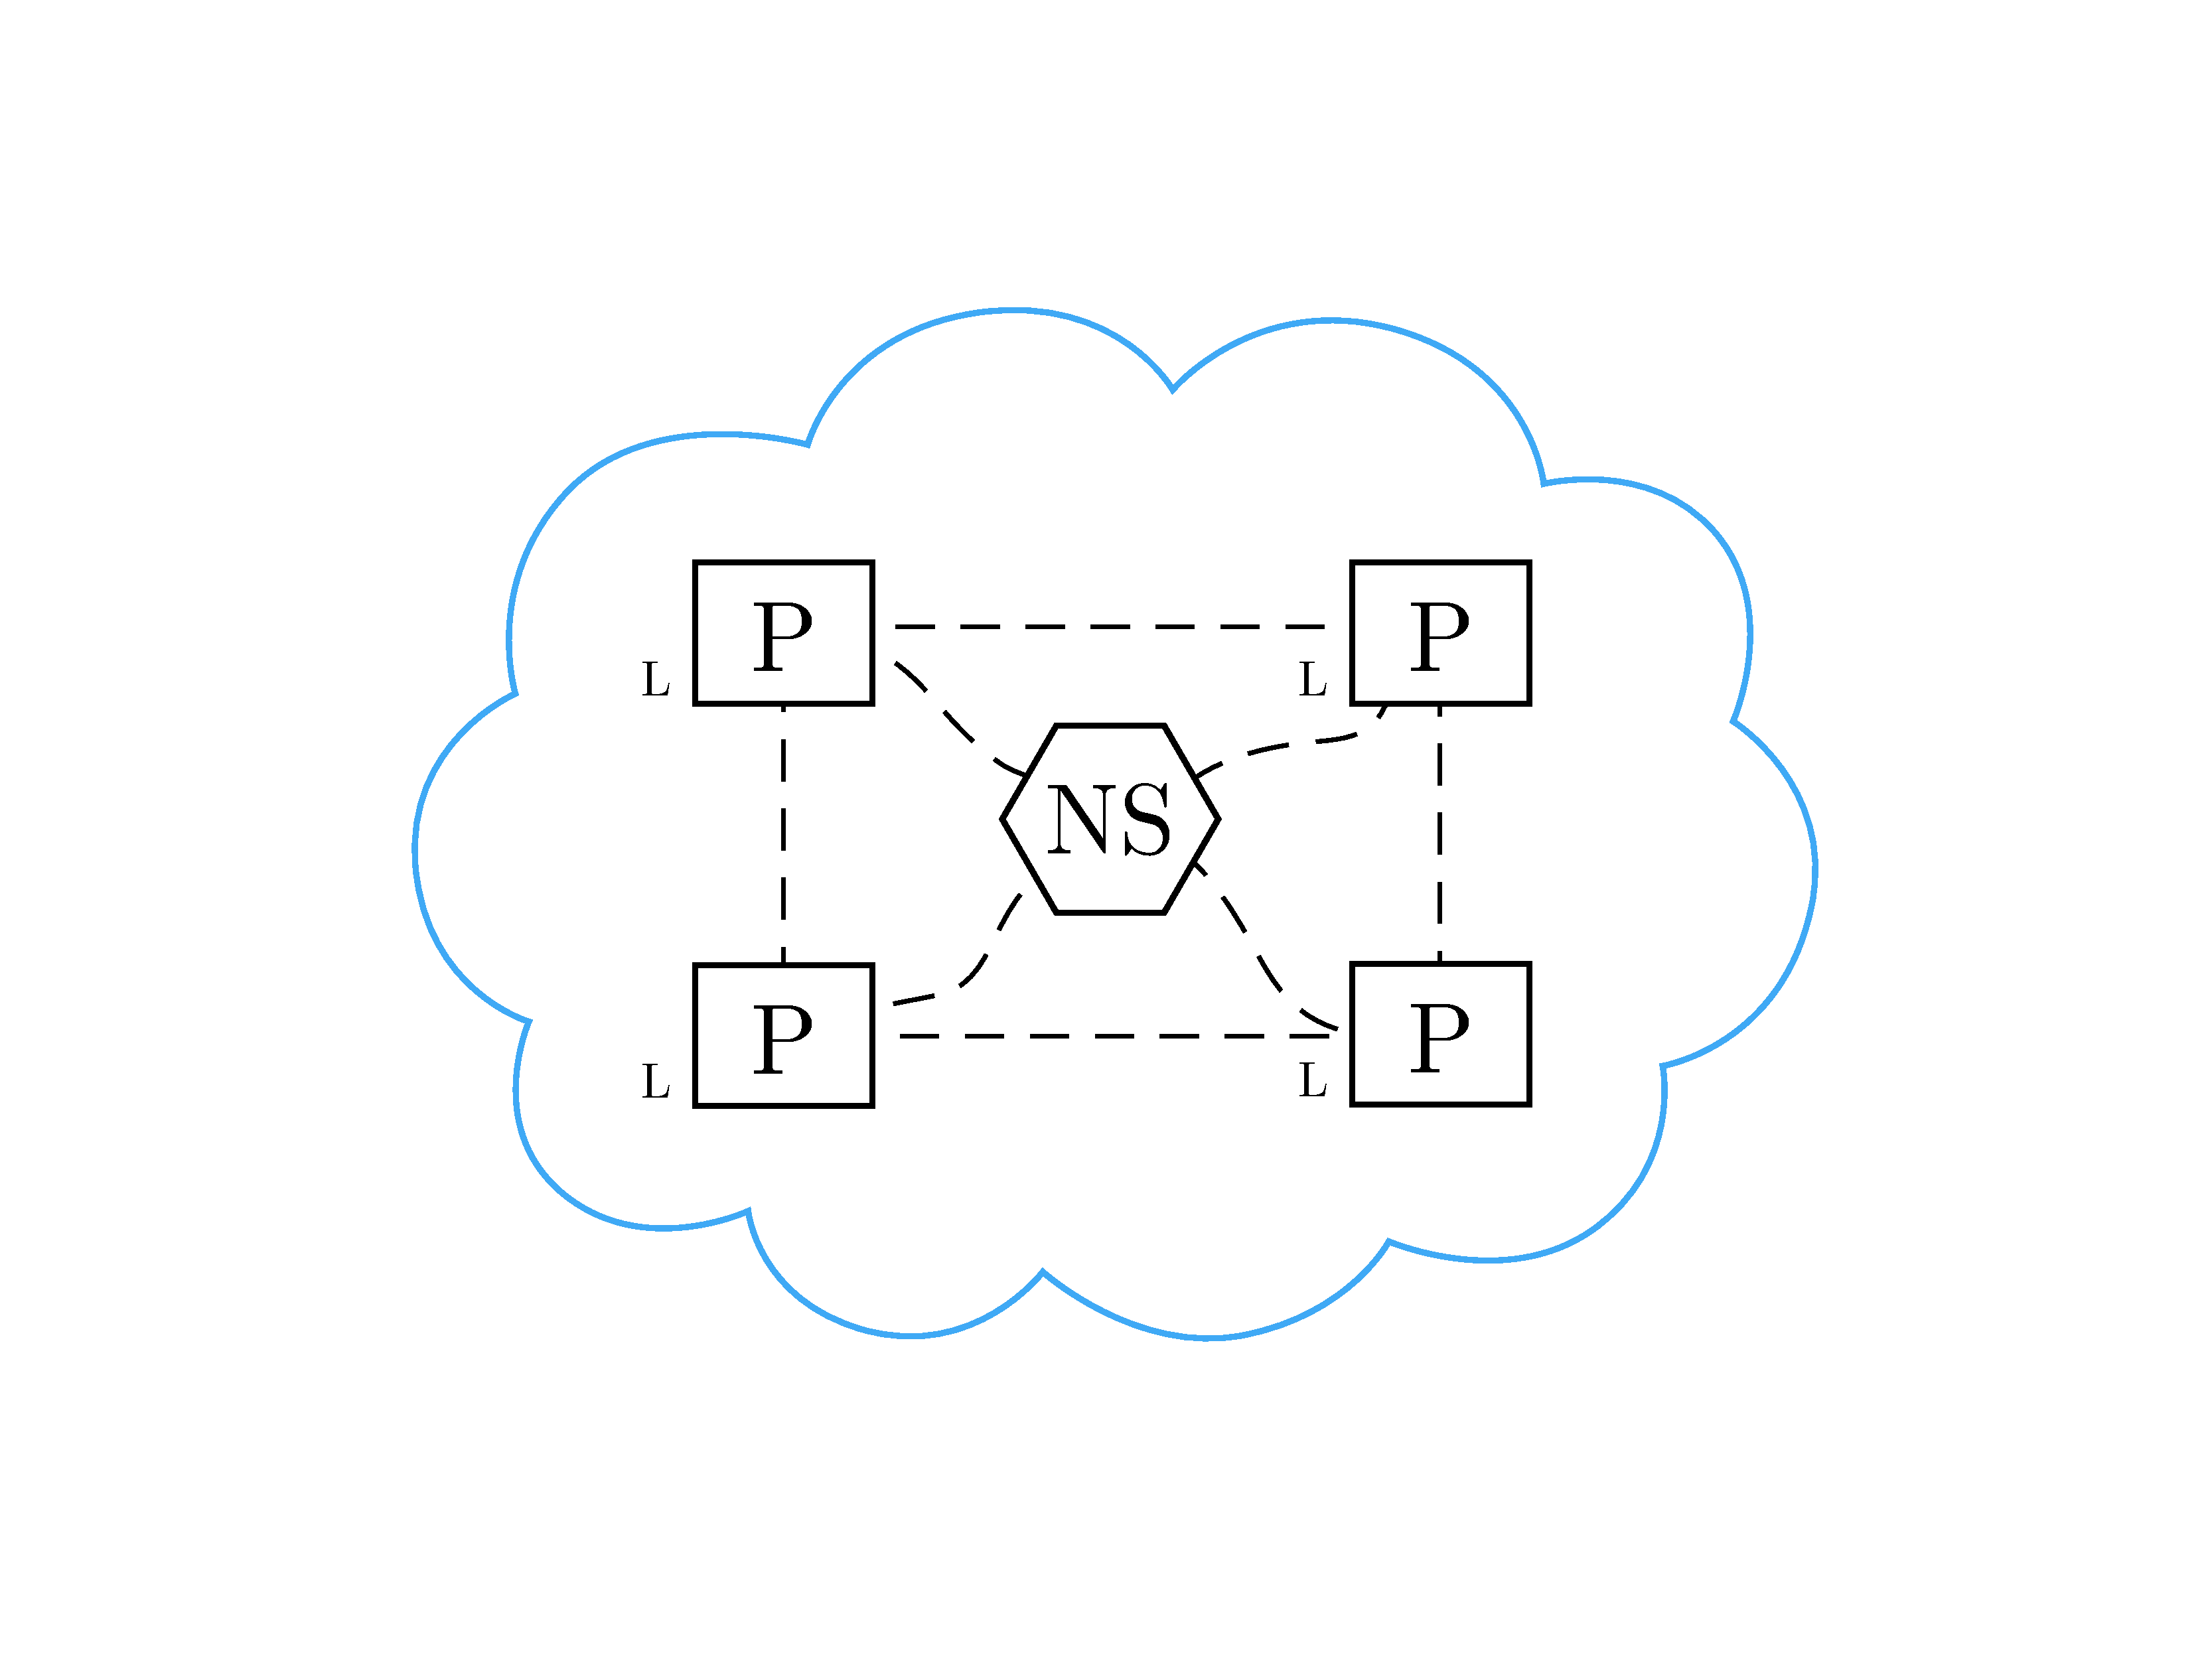
\includegraphics[width=0.8\textwidth, clip=true, trim=0 180px 0 180px]{include/assets/lock.pdf}
  \caption{A name service (NS) and several peers (P) enhanced by a distributed locking mechanism (L).}
  \flabel{lock}
\end{figure}

The database of fortunes that you are developing in this programming project is
an example of a resource which is distributed across a network. Eventually, each
peer will have a local copy of the data, and this copy will be kept consisted
with all other copies. Having achieved this goal, any client/user connected to
the database of any peer will see the same data, and any operation performed on
these data will be automatically propagated to all other peers and, thus, to all
other clients. As this point, it might be helpful to have a look at the first
illustration given in the documentation for \aref{0}. It is apparent that
several peers might try to access shared resources simultaneously. Thus, such
resources have to be protected in order to eliminate corrupted states of the
data.

The goal for this assignment is to implement an algorithm for distributed mutual
exclusion, which will address the aforementioned concern. This locking-enhanced
configuration of the system is depicted in \fref{lock}. More specifically, we
shall focus on the second Ricart--Agrawala algorithm \cite{lecture67} (the one
based on tokens). In a nutshell, using this algorithm, peers will be able to
uniquely determine which of them is allowed to enter its critical section, \ie,
to operate on the shared resource. This will be achieved by virtue of a
so-called token, which will be passed between the peers according to a certain
strategy.

Your foremost task is to get yourself familiar with the Ricart--Agrawala
algorithm by reading the corresponding lecture notes. Apart from the material
given in \cite{lecture67}, you might also want to refresh your knowledge on
logical clocks described in \cite{lecture5} as they are an essential part of the
algorithm.

\section{Your Task}
\subsection{Preparation}
Continue working with the same code base that you have been working with so far,
including all the changes that you have made. The files relevant to this
assignment are listed below. You should read and understand them.
\begin{itemize}

  \item \filename{lab4/mutexPeer.py} --- the main application (\leave);

  \item \filename{lab4/test.sh} --- a shell script that you can use for testing;

  \item \filename{modules/Common/nameServiceLocation.py} --- the same as for
  \aref{2} (\leave);

  \item \filename{modules/Common/objectType.py} --- the same as for \aref{2}
  (\overwrite);

  \item \filename{modules/Common/orb.py} --- the same as for \aref{2}
  (\overwrite);

  \item \filename{modules/Common/wrap.sh} --- the same as for \aref{1};

  \item \filename{modules/Server/peerList.py} --- the same as for \aref{3}
  (\overwrite);

  \item \filename{modules/Server/lock/distributedLock.py} --- the distributed
  lock (\fix).

\end{itemize}
As usual, you should reuse your implementations from the previous assignments
and overwrite the corresponding files listed above.

Carefully go through the code in \filename{mutexPeer.py} and
\filename{distributedLock.py}. The former is the main executable file of this
assignment. It is a simple test application serving the only purpose of
acquiring and releasing the distributed lock in \filename{distributedLock.py} by
choosing the corresponding commands from the menu of the application (see
below). Run several instances of \filename{mutexPeer.py} in parallel and try to
acquire the lock in all of them simultaneously:
\begin{shell}
\$ ./mutexPeer.py -t ivan
Choose one of the following commands:
    l  ::  list peers,
    s  ::  display status,
    a  ::  acquire the lock,
    r  ::  release the lock,
    h  ::  print this menu,
    q  ::  exit.
ivan(0):RELEASED> a
Trying to acquire the lock...
ivan(0):LOCKED>
...
ivan(1):LOCKED>
...
ivan(2):LOCKED>
...
\end{shell}
As you can see, all the peers have successfully entered their critical sections
at the same time; in other words, our distributed lock does not work.

\subsection{Implementation}
Your task is to implement the second Ricart--Agrawala algorithm for distributed
mutual exclusion. Read the description of the algorithm given in
\cite{lecture67} and complete the following functions of the
\classname{DistributedLock} class:
\begin{itemize}

  \item \code{initialize} --- the function initializes the state of the lock for
  the current peer based on a populated peer list; make sure that the token is
  initially granted to only one peer.

  \item \code{destroy} --- called when the current peer leaves the system; if
  the peer has the token, it passes the token to somebody else.

  \item \code{register\_peer} --- called when some other peer (not the current
  one) joins the system; the newcomer should be properly taken into account.

  \item \code{unregister\_peer} --- called when some other peer (not the current
  one) leaves the system; the quitter should be excluded from consideration.

  \item \code{acquire} --- called when the current peer tries to acquire the
  lock; if the token is not present, the peer should notify the rest about its
  desire and suspend its execution until the token is passed to the peer.

  \item \code{release} --- called when the current peer releases the lock; if
  there are peers waiting for the token, the current peer should pass the token
  to one of them (carefully think through to whom in order to ensure fairness).

  \item \code{request\_token} --- called when some other peer requests the token
  from the current peer (should the current one have the token or not).

  \item \code{obtain\_token} --- called when some other peer gives the token to
  the current peer; if the current peer is waiting for the token (and, thus, its
  execution is suspended in \code{acquire}), it should resume its execution.

\end{itemize}
Make sure that the algorithm properly handles situations when peers dynamically
join and leave the system. For simplicity, you may assume that the peer holding
the token never disappears (\eg, due to a system crash) without passing the
token to someone else.

\section{Conclusion}
In this assignment, you have implemented one of the algorithms for distributed
mutual exclusion. As motivated in the introduction, such an algorithm is a
crucial component of a distributed system as it makes it possible to maintain
shared resources in consistent states. The final step is to integrate all the
components that you have implemented so far into a robust distributed database,
in which an arbitrary number of peers will be maintaining the content of the
database, and an arbitrary number of clients/users will be able to seamlessly
connect to this database and to safely perform all the needed operations.

\printbibliography

\end{document}

% vim: ft=tex
